\section{Introduction}
This chapter describes the methodology adopted to develop the proposed explainable deep learning framework for skin condition classification and severity estimation. The methodology consists of dataset collection, preprocessing, transfer learning model development, training, prediction, explainability, and performance evaluation. Three pre-trained convolutional neural network architectures, namely EfficientNetB0, MobileNetV2, and ResNet50, were implemented and comparatively evaluated. Grad-CAM was incorporated to provide visual explanations of the model's predictions, improving transparency and interpretability.

\section{Research Framework}
The proposed framework follows a sequential workflow beginning with dataset collection and preprocessing. The dataset is then divided into training, validation, and testing subsets before applying data augmentation techniques. Three transfer learning models are trained independently using the prepared dataset. After training, each model predicts the probabilities of all skin condition–severity labels. Finally, Grad-CAM visualization is generated to highlight the image regions contributing to the model's predictions, followed by quantitative performance evaluation and comparative analysis.

\section{Dataset Collection}
The dataset used in this study consists of 8,275 images grouped into four categories: Acne \cite{Ansari2026SkinDataset}, Burn \cite{ShubhamBaidSkinBurnDataset}, Eczema \cite{Ansari2026SkinDataset}, and Normal \cite{ShakyaSkinTypesDataset} skin. The Acne, Burn, and Eczema categories each contain three severity levels: Mild, Moderate, and Severe. The Normal skin category contains three skin types: Dry, Normal, and Oily, resulting in a total of 12 labels. All images were resized to a uniform resolution of \(224 \times 224\) pixels with three color channels (RGB) to maintain consistency across the dataset.

\begin{figure}[htbp]
    \centering
    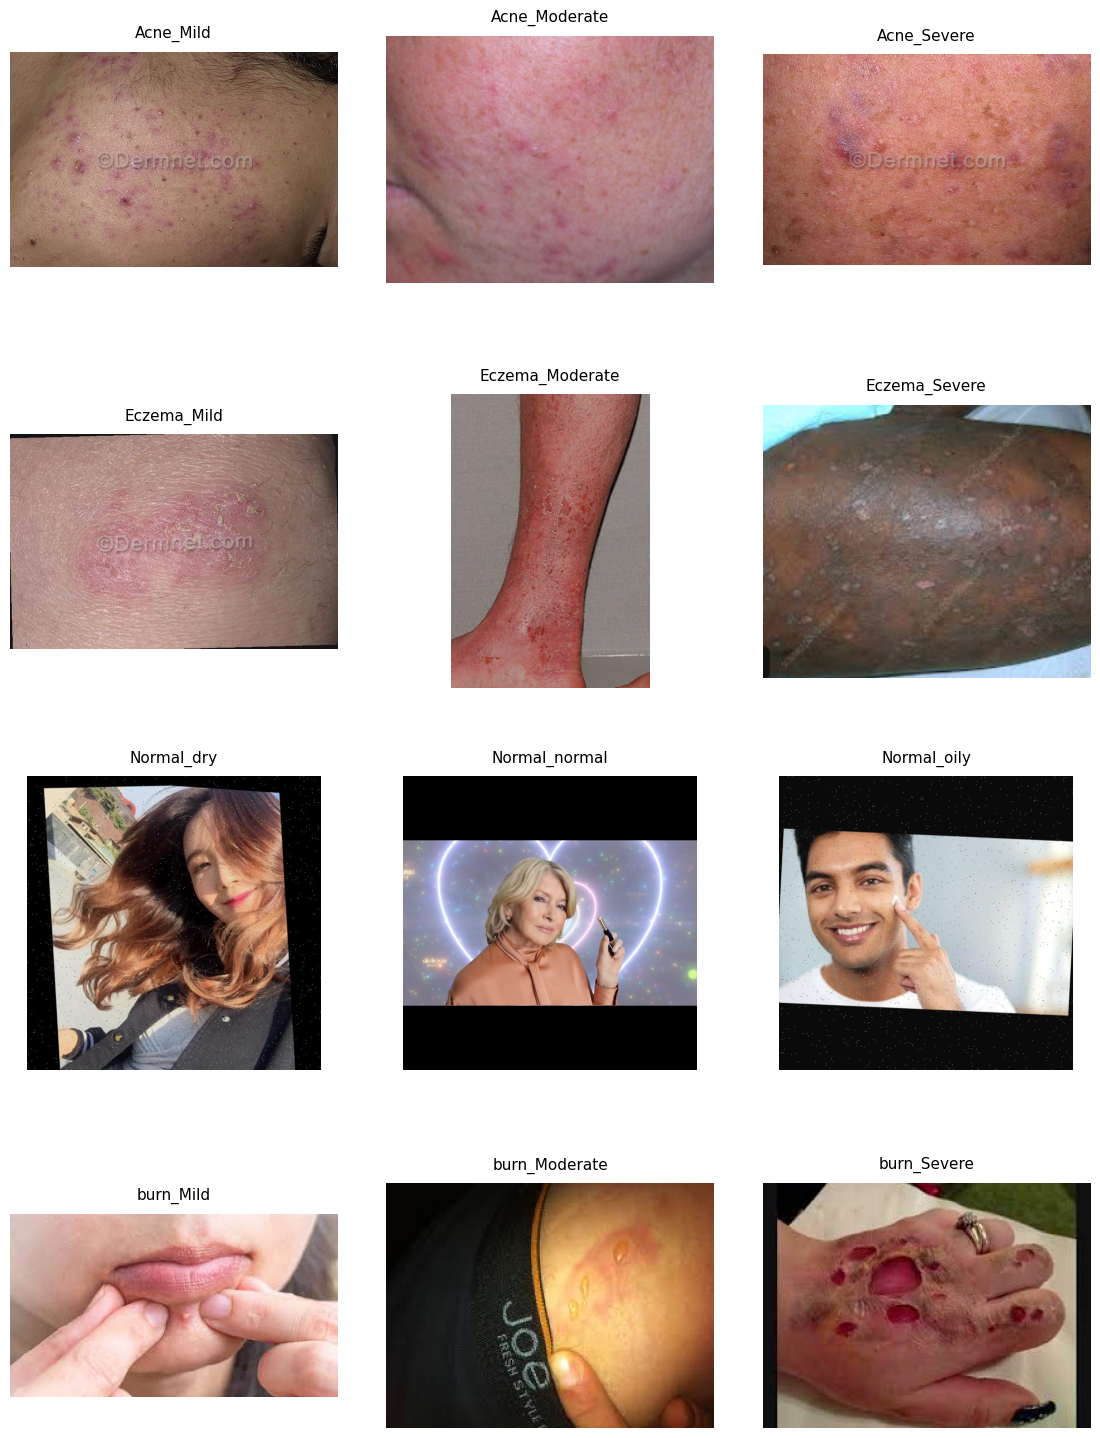
\includegraphics[width=0.9\textwidth]{images/dataset_sample.png}
    \caption{Representative Images of Skin Conditions and Their
    Corresponding Severity Levels in the Dataset}
    \label{fig:skin_dataset_samples}
\end{figure}

To support systematic data management and model development, the dataset was organized into structured folders, and metadata containing image paths, labels, category information, and corresponding severity levels or skin types was generated automatically. This metadata was used to map the 12 labels to unique numerical indices and facilitate consistent data loading, preprocessing, training, and evaluation.


\section{Data Preprocessing}
Data preprocessing was performed to ensure consistency in image dimensions, color channels, and label representation before model training. All images were resized to \(224 \times 224\) pixels while preserving three color channels (RGB). Metadata was generated automatically to record image paths, label names, and their corresponding numerical indices, supporting consistent data loading and label mapping throughout the training and evaluation processes.

The dataset contains 12 labels covering three severity levels each for Acne, Burn, and Eczema, along with three Normal skin types: Dry, Normal, and Oily. Each label was assigned a unique numerical index to support the model's output representation. Image validation was also performed to identify and exclude invalid image files, helping maintain dataset integrity.


\section{Dataset Splitting}
The processed dataset was divided into three mutually exclusive subsets using different training proportions, ranging from 60\% to 90\%. For each configuration, the remaining data was divided equally between the validation and test sets. The evaluated configurations were as follows:

\begin{itemize}
\item Training Set: 60\%, Validation Set: 20\%, Test Set: 20\%
\item Training Set: 70\%, Validation Set: 15\%, Test Set: 15\%
\item Training Set: 80\%, Validation Set: 10\%, Test Set: 10\%
\item Training Set: 90\%, Validation Set: 5\%, Test Set: 5\%
\end{itemize}

The training set was used to optimize the model parameters, while the validation set was used to monitor model performance during training, support model selection, and guide adjustments to the training process. The test set was reserved for evaluating model performance on data not used for training or validation. These configurations were investigated to assess how different training data proportions affected classification performance and to identify a suitable dataset split for the proposed framework. For fair comparison among the three transfer learning models, the same split configuration and corresponding data partitions were used when comparing the models under each experimental setting.


\section{Data Augmentation}
To improve model generalization and reduce overfitting, data augmentation techniques were applied to the training dataset. The augmentation process included horizontal flipping only.\\
This transformation generated diverse training samples while preserving the semantic characteristics of the skin conditions. Validation and test datasets were not augmented to ensure unbiased evaluation.

\section{Proposed Deep Learning Framework}
The proposed framework employs transfer learning to adapt pre-trained convolutional neural network architectures for skin condition classification and severity estimation. Instead of training the networks from scratch, ImageNet-pretrained models are used as feature extractors and adapted to the target dataset. Data augmentation and model-specific preprocessing are applied to the input images before feature extraction.

A custom classification head is added to the backbone network. It consists of a Global Average Pooling layer, Batch Normalization, a Dropout layer with a rate of 0.30, a fully connected Dense layer containing 256 units with Swish activation and L2 regularization, a second Dropout layer with a rate of 0.30, and an output layer containing 12 units. The output layer uses sigmoid activation to produce an individual score for each skin-condition.

The models are compiled using the Binary Cross-Entropy loss function and the selected optimizer. The sigmoid activation and Binary Cross-Entropy loss support independent output scores for the labels, provided that the target encoding is consistent with a multilabel learning formulation. These scores allow the model's predictions to be examined across all 12 labels rather than displaying only the highest-scoring label.


\section{Transfer Learning Models}
Three pre-trained convolutional neural network architectures were selected for comparison:
\begin{itemize}
    \item EfficientNetB0
    \item MobileNetV2
    \item ResNet50
\end{itemize}

These models were chosen because they employ different architectural approaches to feature extraction and computational efficiency, allowing their suitability for skin condition classification and severity estimation to be evaluated.

EfficientNetB0 uses a compound scaling strategy to balance network depth, width, and input resolution, making it a suitable candidate for investigating the trade-off between classification performance and computational cost. MobileNetV2 employs inverted residual blocks and linear bottlenecks to reduce computational requirements, making it useful for evaluating inference efficiency. ResNet50 uses residual connections to facilitate the training of deeper networks and learn complex visual features, providing a contrasting approach for skin image analysis.

Each model was initialized using ImageNet pre-trained weights. During the first training stage, the feature extraction layers were frozen while only the newly added classification layers were trained. During the second stage, selected layers of the backbone network were unfrozen and fine-tuned using a smaller learning rate to improve task-specific feature learning.\\
The performance of all three architectures was compared using identical preprocessing, training, and evaluation procedures.

\section{Model Training}
The models were trained using the TensorFlow and Keras deep learning framework. Early stopping and model checkpointing were employed to prevent overfitting and preserve the best-performing model based on validation performance.\\
The Adam optimizer was used for optimization with adaptive learning rate scheduling. ReduceLROnPlateau automatically decreased the learning rate whenever validation performance stopped improving, allowing the model to converge more effectively.\\
Training performance was monitored using training and validation accuracy together with training and validation loss.

\section{Prediction and Severity Estimation}
After training, each model predicts confidence scores for all skin condition–severity labels simultaneously. The prediction results are organized according to their corresponding skin conditions, allowing users to observe the confidence associated with every severity level.\\
The predicted confidence scores provide a comprehensive assessment rather than only displaying the highest predicted class. This information may assist in monitoring changes in skin condition severity across multiple observations captured during different stages of treatment.

\section{Explainability Using Grad-CAM}
To improve transparency, Gradient-weighted Class Activation Mapping (Grad-CAM) was integrated into the proposed framework. Grad-CAM generates heatmaps highlighting the regions of the input image that contribute most significantly to each predicted label.\\
Unlike conventional classification systems that provide only prediction scores, Grad-CAM allows users to visualize the evidence supporting the model's decisions. This improves the interpretability of the framework and increases user confidence in automated predictions.

\section{Performance Evaluation}
The proposed models were evaluated using the independent test dataset. Performance was assessed using several evaluation metrics, including Accuracy, Precision, Recall, and F1-score.\\
In addition to numerical evaluation, confusion matrices and classification reports were generated to analyze model performance for individual classes. The three transfer learning architectures were then comparatively analyzed to determine the most suitable model for the proposed skin condition classification framework.

\section{Chapter Summary}
This chapter presented the methodology used to develop the proposed explainable transfer learning framework for skin condition classification and severity estimation. The methodology covered dataset preparation, preprocessing, transfer learning model development, training, prediction, Grad-CAM visualization, and performance evaluation. The following chapter presents the experimental results and comparative analysis of the proposed models.